% !TEX root = report.tex
\section{Analysis}

\begin{figure}[]
\centering
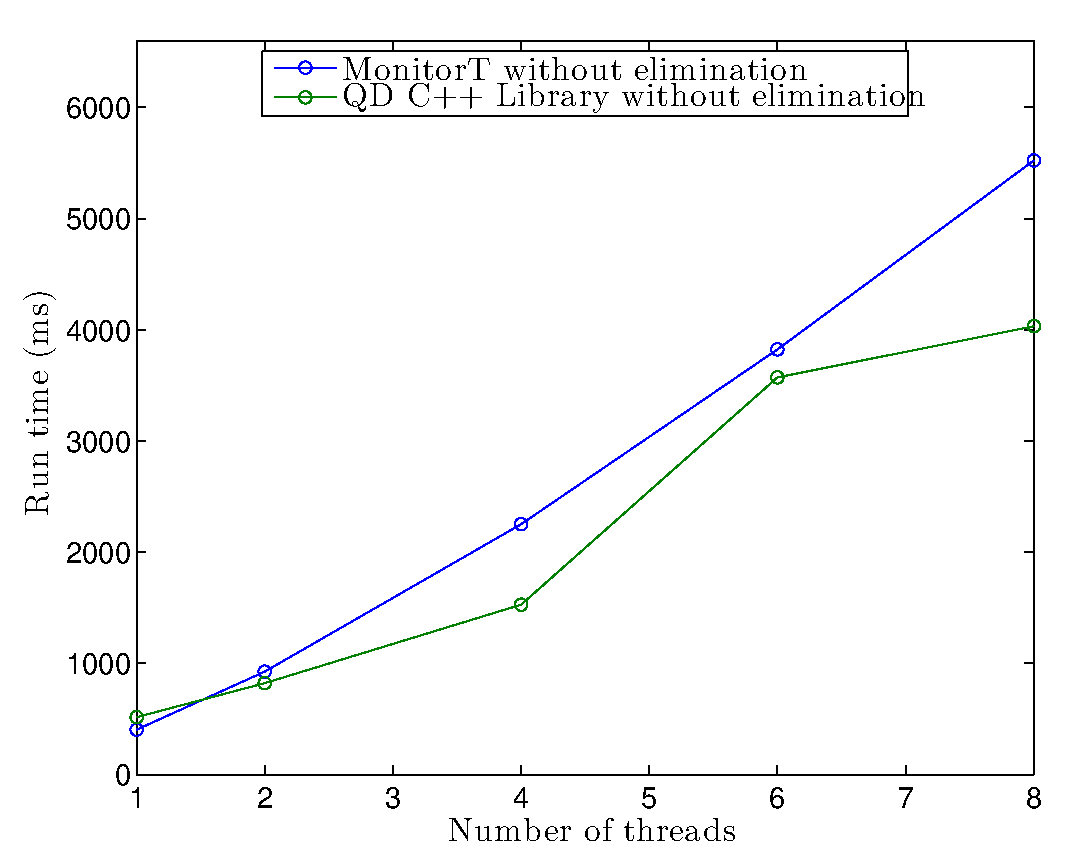
\includegraphics[width=.75\textwidth]{figs/00_TimeVsThreads_cppNoElim_javaNoElim.eps}
\caption[]{Baseline comparison of the MonitorT implementation (Java) and the QD Lock (C++), varying the number of threads, and without elimination for either implementation. Queue size = 256, push ratio is 0.5.}
\label{fig:fig00}
\end{figure}

\begin{figure}[]
\centering
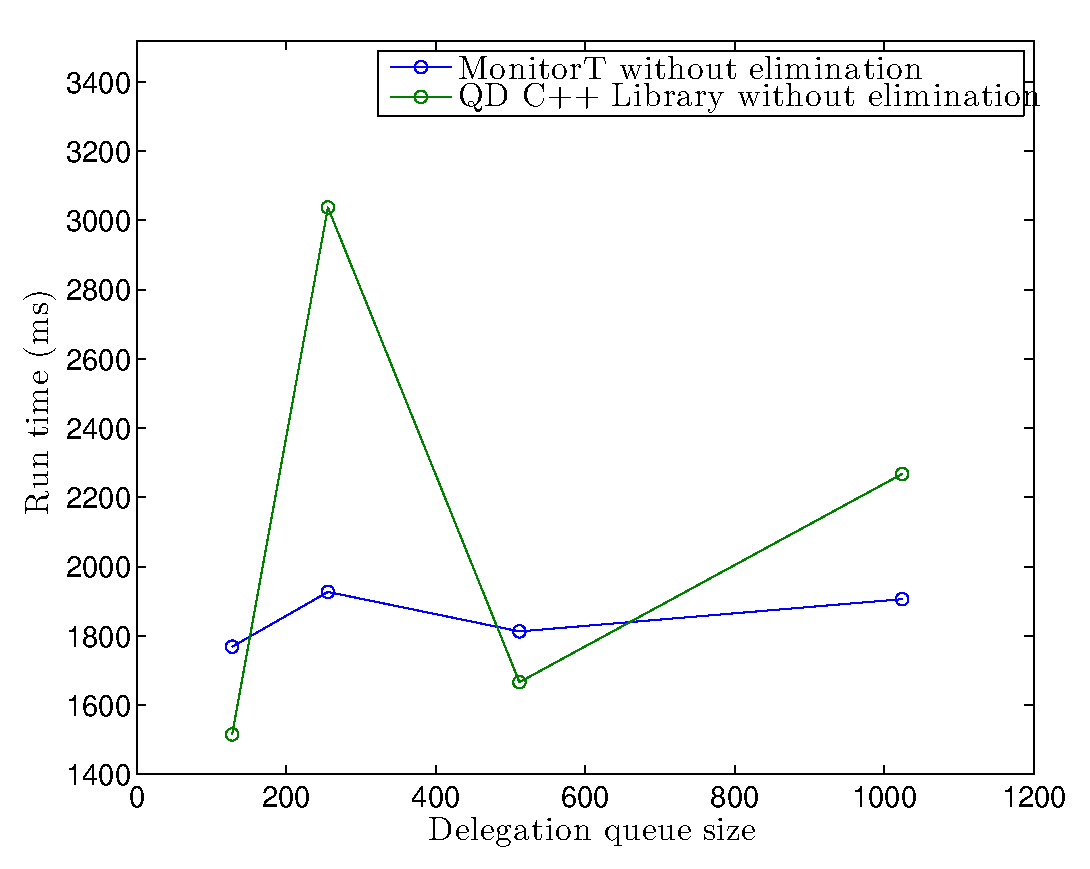
\includegraphics[width=.75\textwidth]{figs/01_TimeVsQDsize_cppNoElim_javaNoElim.eps}
\caption[]{Baseline comparison of the MonitorT implementation (Java) and the QD Lock (C++), varying the delegation queue size, and without elimination for either implementation. Threads = 4, push ratio = 0.5.}
\label{fig:fig01}
\end{figure}

\begin{figure}[]
\centering
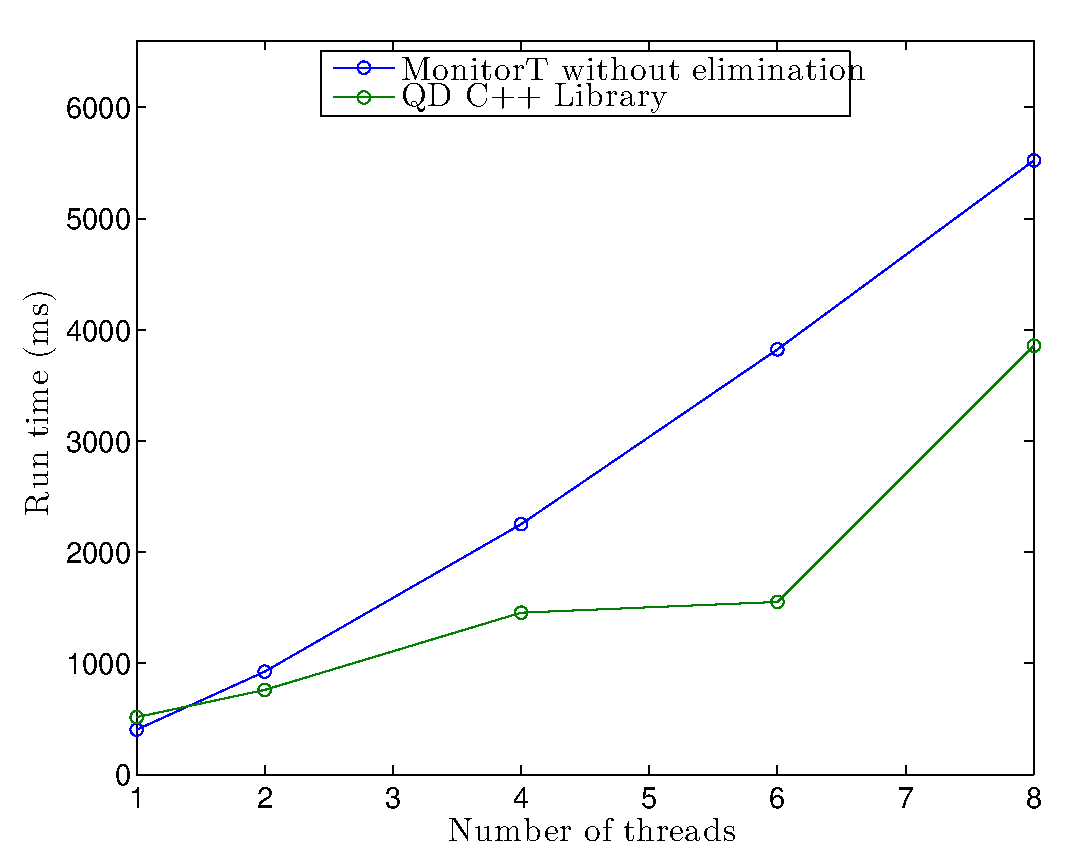
\includegraphics[width=.75\textwidth]{figs/02_TimeVsThreads_cppElim_javaNoElim.eps}
\caption[]{Comparison of the MonitorT implementation (Java) and the QD Elimination Lock (C++), varying the number of threads (elimination included for C++ implementation, not for Java). Queue size = 256, push ratio is 0.5.}
\label{fig:fig02}
\end{figure}

\begin{figure}[]
\centering
\subfloat[][]{\label{fig:fig03}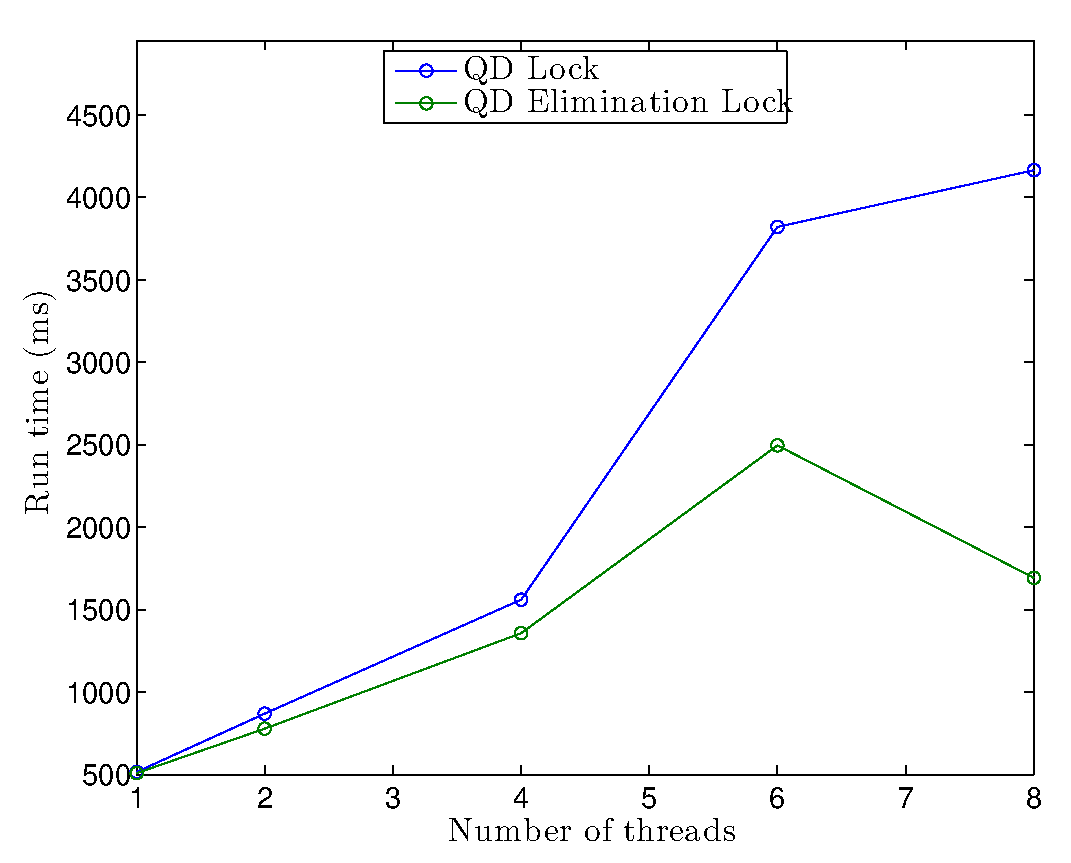
\includegraphics[width=.49\textwidth]{figs/03_TimeVsThreads_cppElim_cppNoElim.eps}}
\subfloat[][]{\label{fig:fig04}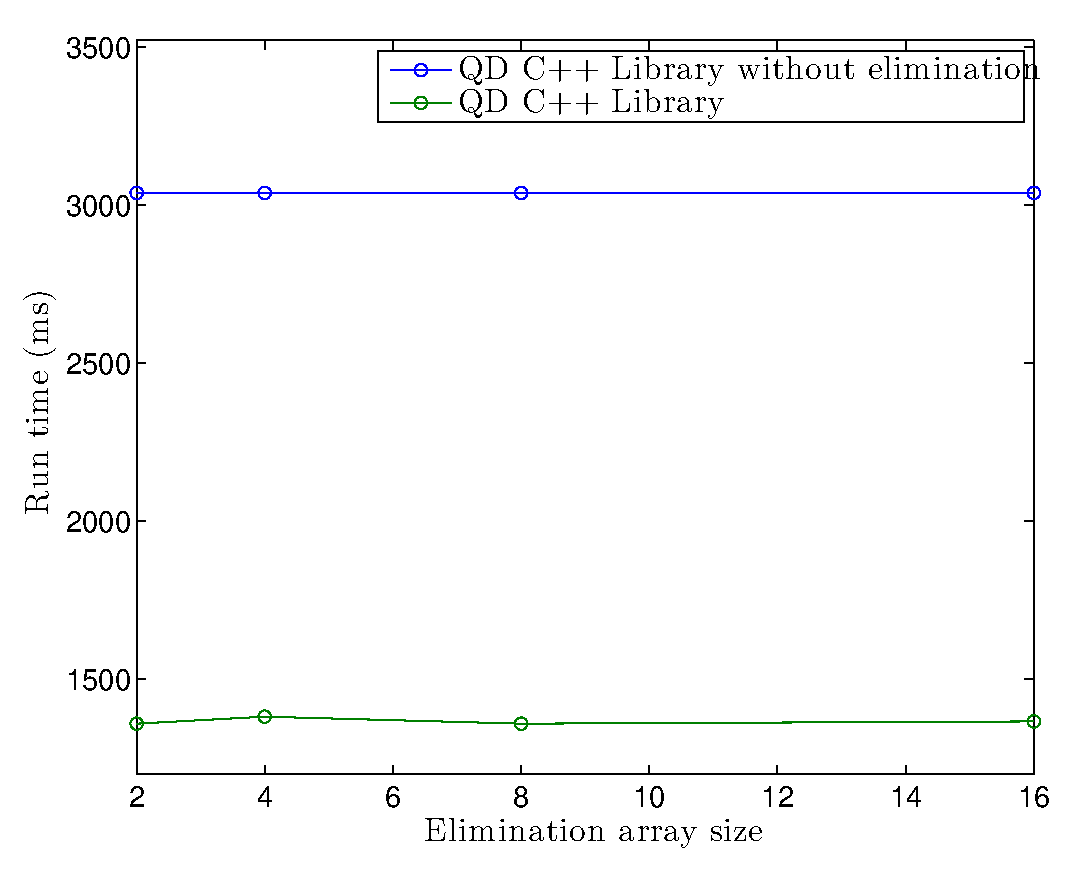
\includegraphics[width=.49\textwidth]{figs/04_TimeVsElsize_cppElim_cppNoElim.eps}}\\
\subfloat[][]{\label{fig:fig05}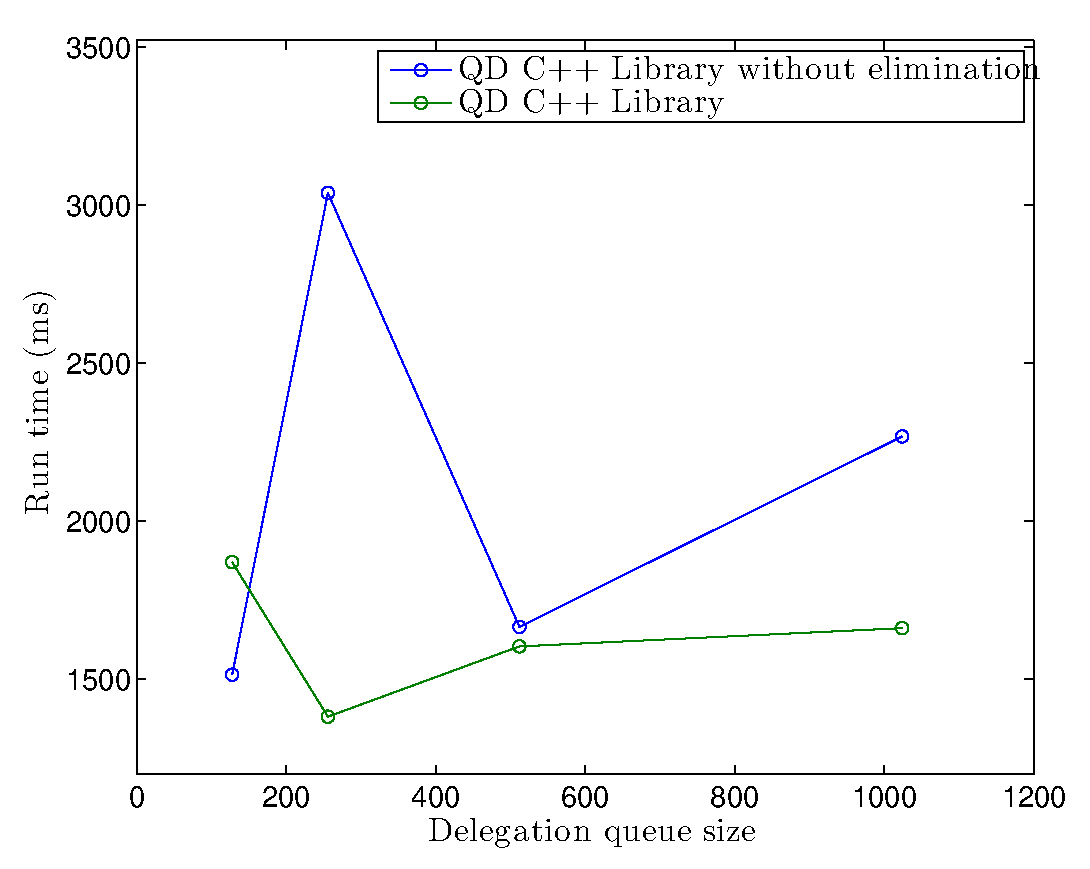
\includegraphics[width=.49\textwidth]{figs/05_TimeVsQDsize_cppElim_cppNoElim.eps}}
\subfloat[][]{\label{fig:fig06}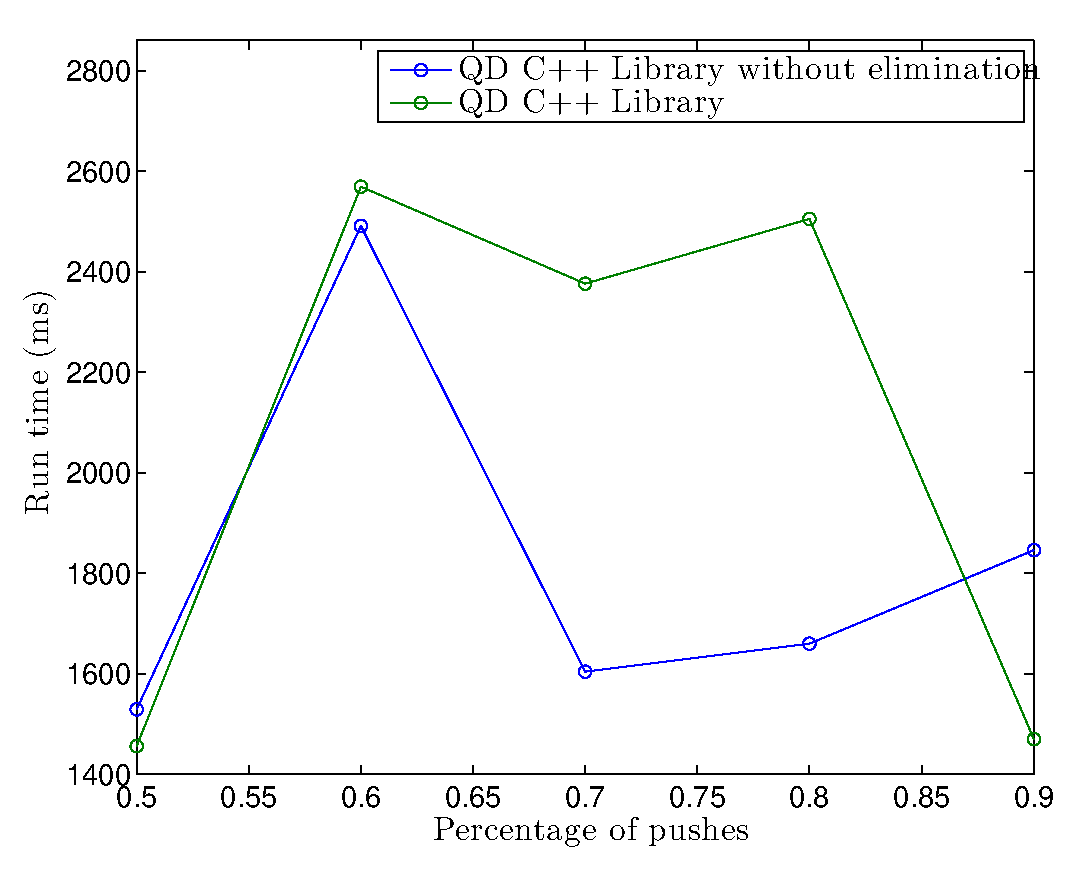
\includegraphics[width=.49\textwidth]{figs/06_TimeVsPctPush_cppElim_cppNoElim.eps}}
\caption[]{QD Elimination Lock versus QD Lock (both C++): \subref{fig:fig03} varying the number of threads (elimination array size = 4, queue size = 256, push ratio = 0.5); \subref{fig:fig04} varying the elimination array size (threads = 4, queue size = 256, push ratio = 0.5); \subref{fig:fig05} varying the delegation queue size (threads = 4, elimination array size = 4,push ratio = 0.5); \subref{fig:fig06} varying the push ratio (threads = 4, elimination array size = 4, queue size = 256).}
\label{fig:final}
\end{figure}

\begin{figure}[]
\centering
\subfloat[][]{\label{fig:fig07a}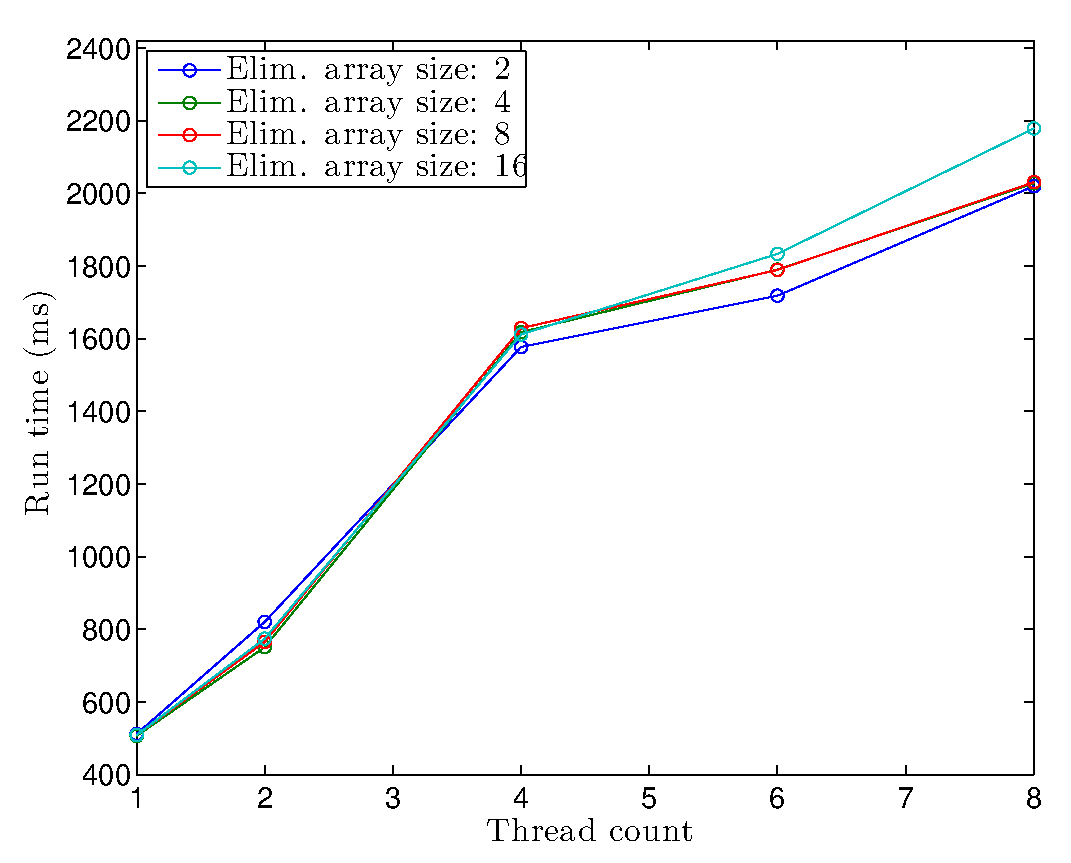
\includegraphics[width=.49\textwidth]{figs/07a_Q128_TimeVsThreadsVsEsize_cppElim.eps}}
\subfloat[][]{\label{fig:fig07b}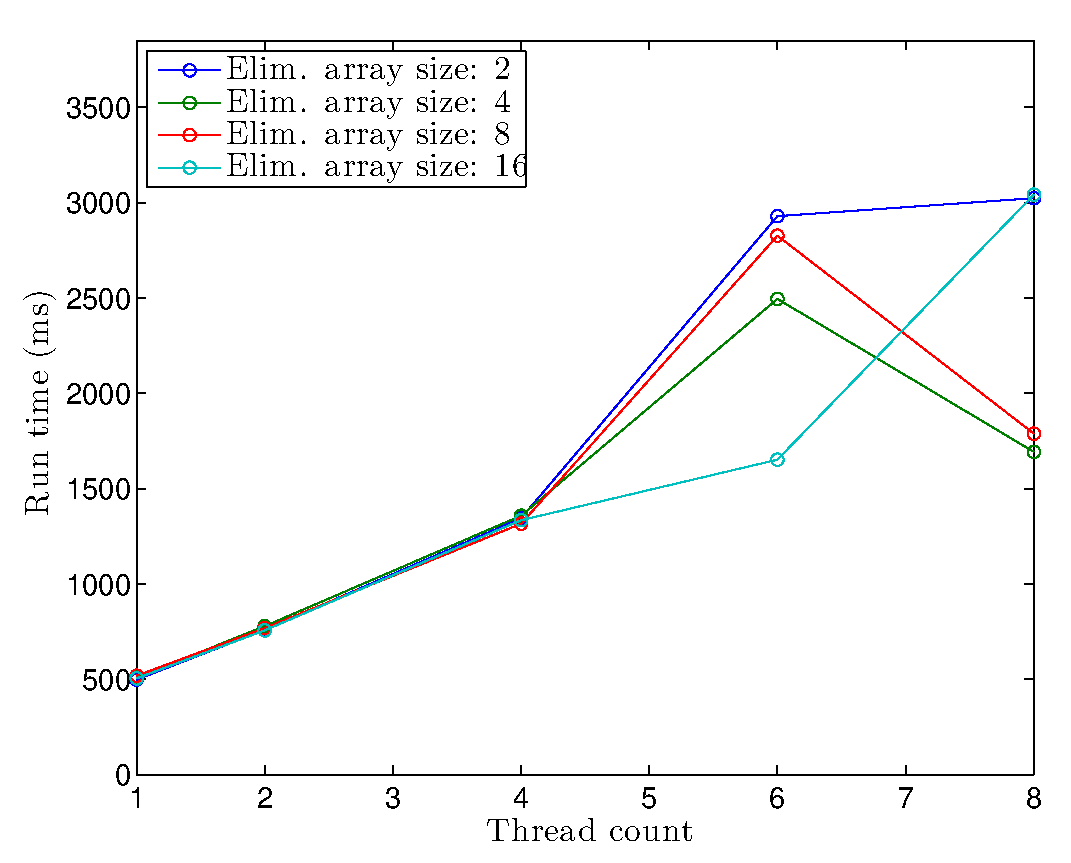
\includegraphics[width=.49\textwidth]{figs/07b_Q256_TimeVsThreadsVsEsize_cppElim.eps}}\\
\subfloat[][]{\label{fig:fig07c}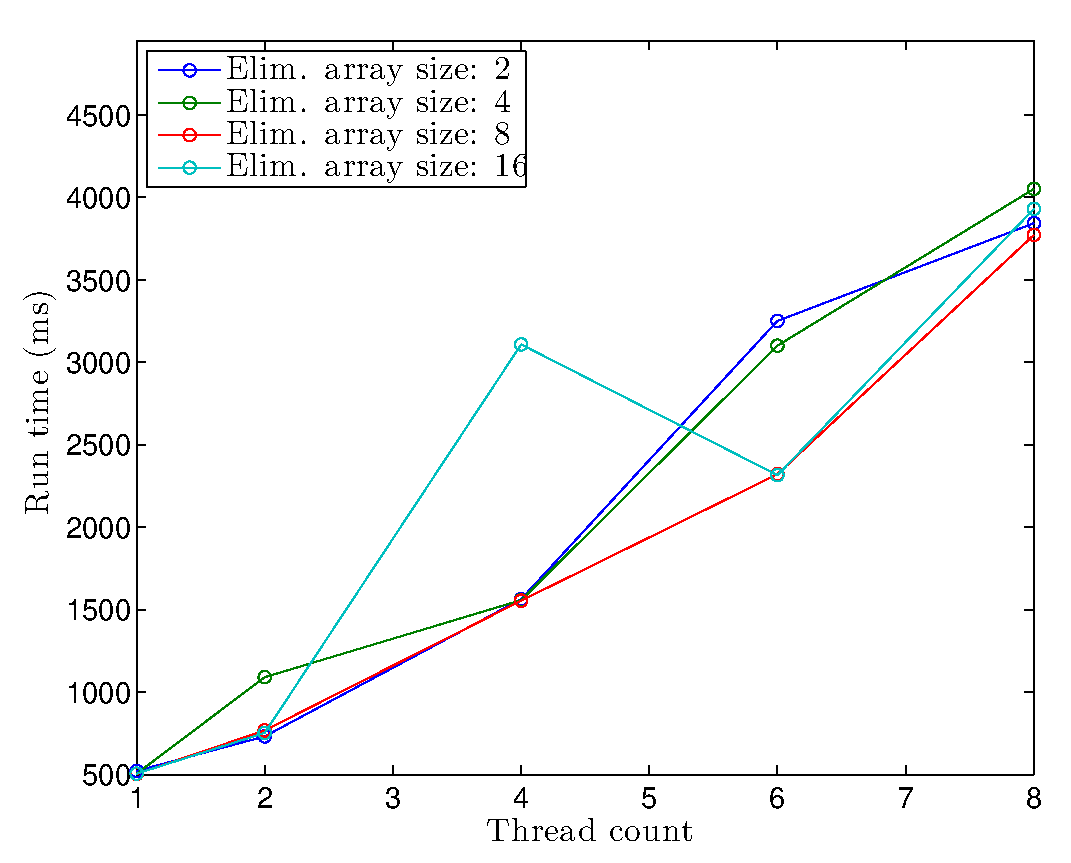
\includegraphics[width=.49\textwidth]{figs/07c_Q512_TimeVsThreadsVsEsize_cppElim.eps}}
\subfloat[][]{\label{fig:fig07d}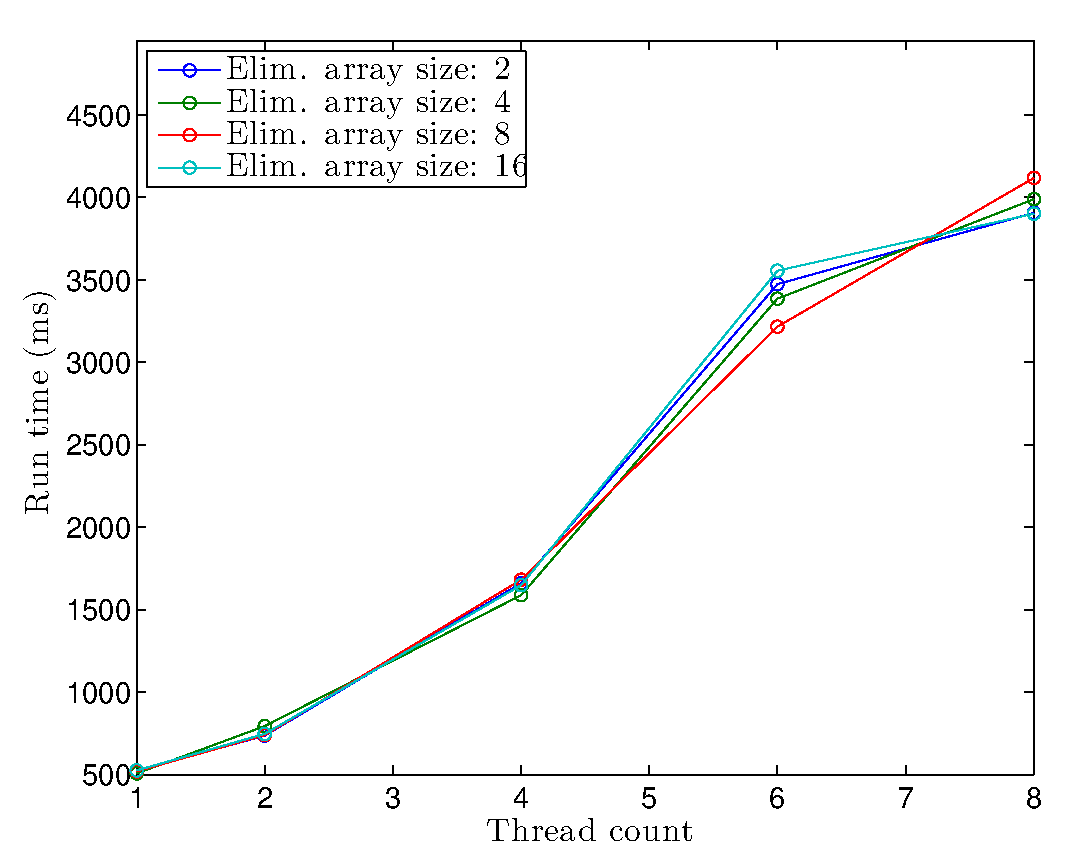
\includegraphics[width=.49\textwidth]{figs/07d_Q1024_TimeVsThreadsVsEsize_cppElim.eps}}
\caption[]{caption: \subref{fig:fig07a} caption; \subref{fig:fig07b} caption; \subref{fig:fig07c} caption; \subref{fig:fig07d} caption.}
\label{fig:final}
\end{figure}

\begin{figure}[]
\centering
\subfloat[][]{\label{fig:fig08a}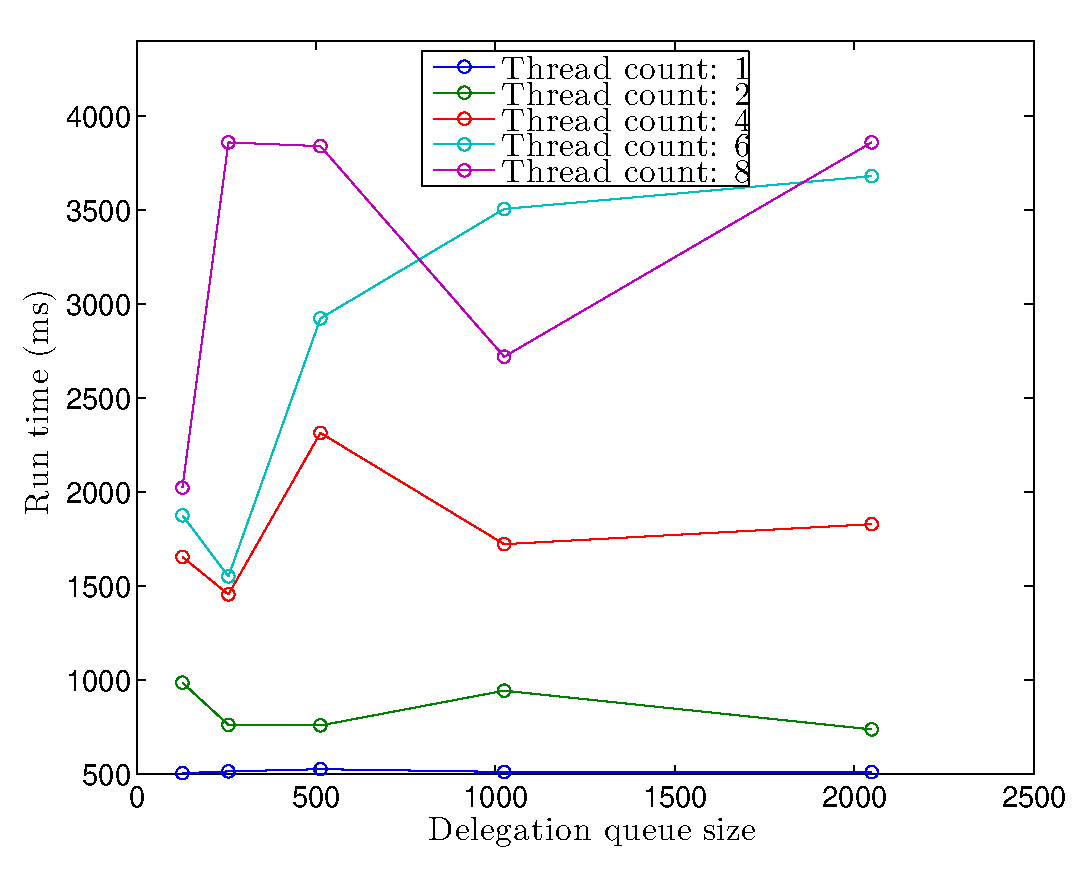
\includegraphics[width=.49\textwidth]{figs/08a_E4_TimeVsEsizeVsThreads_cppElim.eps}}
\subfloat[][]{\label{fig:fig08b}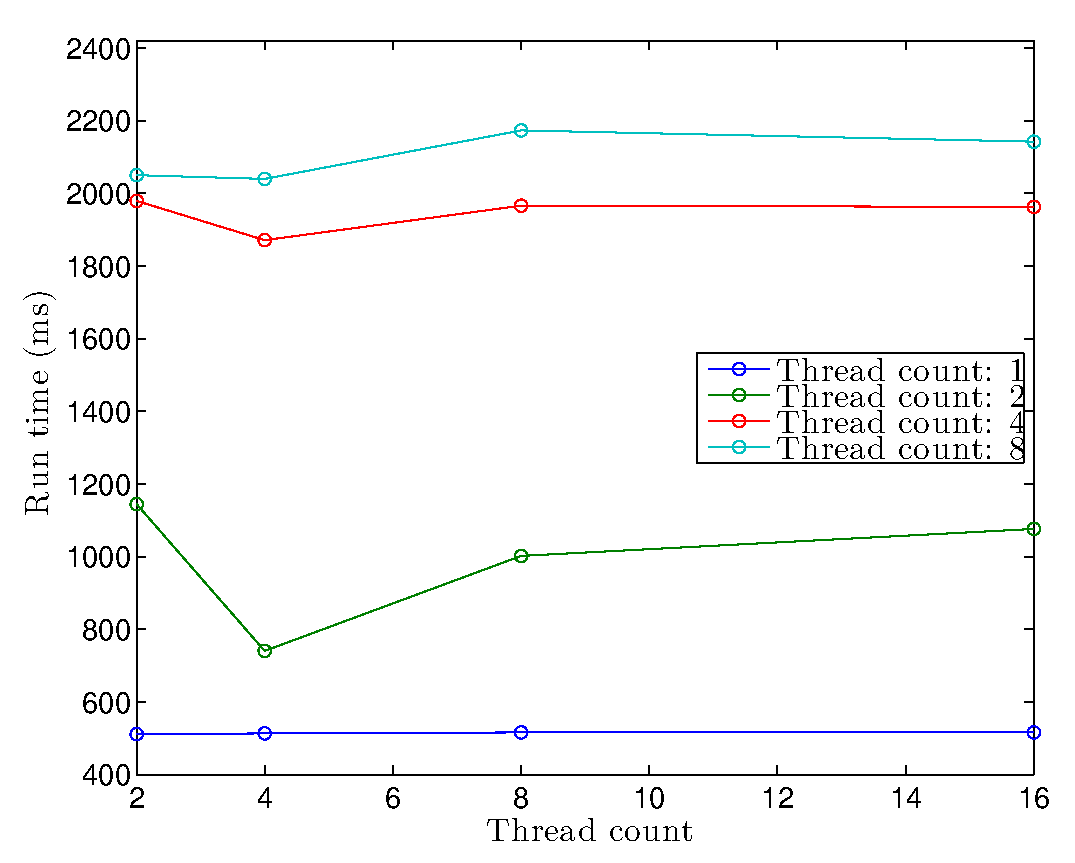
\includegraphics[width=.49\textwidth]{figs/08b_Q128_TimeVsEsizeVsThreads_cppElim.eps}}
\caption[]{caption: \subref{fig:fig08a} caption; \subref{fig:fig08b} caption.}
\label{fig:final}
\end{figure}
